\section{Challenge 3}\label{section:ex3}
%TODO: σχετικο με ch4.
Σε αυτό το challenge προσπαθούμε να μεταβάλουμε τις ταχύτητες του ρομπότ ώστε να ακολουθήσουν ένα δοσμένο μονοπάτι.
Το πρόβλημα ανάγεται στην επιλογή γραμμικής και γωνιακής ταχύτητας δοσμένων της
θέσης $\mathbf{c_R} = \left(x_R, y_R\right)$ και του προσανατολισμού $\theta_R$ του ρομπότ, του επόμενου υποστόχου (σημείο) $\mathbf{c_{sg}} = \left(x_{sg}, y_{sg}\right)$ του μονοπατιού, και των μέγιστων επιτρεπτών ταχυτήτων.
Τα μεγέθη αυτά φαίνονται και στο σχήμα \ref{fig:ex3-coords}.

\begin{figure}[htb]
    \centering
    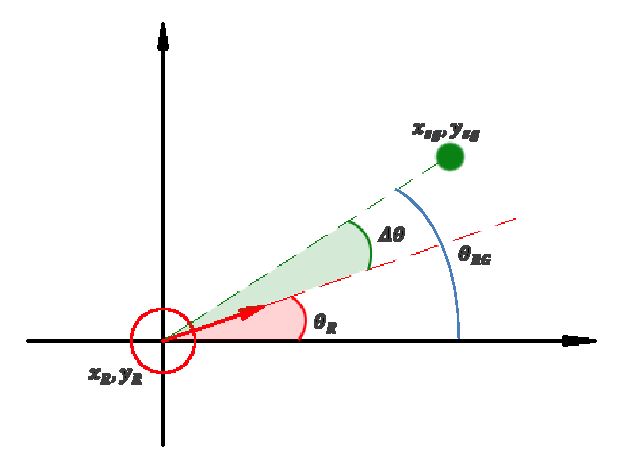
\includegraphics[width=\linewidth]{ex3-coords}
    \caption{Οι θέσεις των σημείων που χρησιμοποιούνται για τον προσδιορισμό των ταχυτήτων. Από~\protect\cite{etsardou-phd}.}\label{fig:ex3-coords}
\end{figure}

Ακολουθείται η διαδικασία που περιγράφεται στην~\cite{etsardou-phd}.
Θεωρούμε ότι τα $x_R$, $y_R$ είναι η αρχή του συστήματος συντεταγμένων και μετασχηματίζουμε τις συντεταγμένες του υποστόχου:
\begin{equation}
    \mathbf{c_{sg}'} = \left(x_{sg}', y_{sg}'\right) = \left(x_{sg} - x_R, y_{sg} - y_R\right)
\end{equation}
και υπολογίζουμε το προσανατολισμό του υποστόχου:
\begin{equation}
    \theta_{sg} = \atantwo{\left(y_{sg}', x_{sg}'\right)}
\end{equation}
Στη συνέχεια, υπολογίζεται ο συντελεστής της γωνιακής ταχύτητας:
\begin{equation}
    \omega = \frac{\Delta{\theta}}{\pi} +
    \begin{cases}
        -2 & \text{Αν $\Delta{\theta} > 0$ και $\Delta{\theta} \geq \pi$} \\
        2  & \text{Αν $\Delta{\theta} < 0$ και $\Delta{\theta} < -\pi$}   \\
        0  & \text{αλλιώς}
    \end{cases}
\end{equation}
ενώ ο συντελεστής της γραμμικής ταχύτητας δίνεται από τη σχέση
\begin{equation}
    u = \left(1-\abs{\omega}^n\right)\label{eq:linear-coeff}
\end{equation}
Η γραμμική ταχύτητα υπολογίζεται έτσι καθώς ο συνδυασμός μεγάλης γραμμικής και γωνιακής ταχύτητας μπορεί να οδηγήσει σε \hyperref[fig:ex3-spiral]{σπειροειδής} κινήσεις του ρομπότ.
Μεγαλύτερες τιμές του $n$ αντιμετωπίζουν πιο ``δραστικά'' το πρόβλημα αλλά μπορεί να οδηγήσουν σε πολύ μικρές γραμμικές ταχύτητες.
Καθώς συναντήσαμε σε μεγάλο βαθμό επιλέξαμε μεγάλη τιμή $n = 6$.
Αυτή η τιμή όμως κάνει το ρομπότ αρκετά αργό και για αυτό το λόγο τροποποιούμε την διαδικασία και επανυπολογίζουμε τον τελικό συντελεστή της γωνιακής ταχύτητας:
\begin{equation}
    \omega' = \sign\left({\omega} \left(1 - u\right)\right)
\end{equation}
Φυσικά, αυτό δεν επηρεάζει τη γραμμική ταχύτητα αλλά κάνει το ρομπότ να στρίβει πιο γρήγορα και να ακολουθεί σχετικά ευθεία τμήματα.

Τέλος οι ταχύτητες υπολογίζονται ως
\begin{equation}
    u_{path} = u \cdot u_{max}
\end{equation}
και
\begin{equation}
    \omega_{path} = \omega \cdot \omega_{max}
\end{equation}

\begin{figure}[htb]
    \centering
    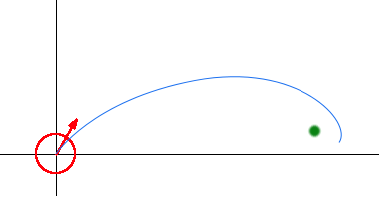
\includegraphics[width=\linewidth]{ex3-spiral}
    \caption{Εκτέλεση σπειροειδούς κίνησης εξαιτίας μεγάλης γραμμικής ταχύτητας. Από~\protect\cite{etsardou-phd}.}\label{fig:ex3-spiral}
\end{figure}

Αποτέλεσμα του path following φαίνεται σε στιγμιότυπο στην εικόνα \ref{fig:random-with-path-following}.
